\documentclass[a4paper,oneside,11pt]{article}

%-----------------------------------------------
% A user manual for the gitLAMMPS repository on Bitbucket owned by the GranLAMMPS team.

% History:
% v1.0		KH - 4 August 2014	Based on user manual for repository in shared space at Imperial
%-----------------------------------------------



%-----------------------------------------------
% Layout and Formatting
%-----------------------------------------------
\usepackage[T1]{fontenc} % Use T1 encoding as the default document encoding.
\usepackage[activate={true,nocompatibility},final]{microtype} % This enables character protrusion (margin kerning) and font expansion.
\usepackage{tgpagella,color,fancyhdr,lastpage,alltt,titlesec,prettyref,graphicx}
\usepackage[normalem]{ulem} % For strikethrough text
\usepackage[font=small,labelfont=bf]{caption}
\usepackage[a4paper,left=2.2cm,right=2.2cm,top=1.2cm,bottom=2.2cm,includeheadfoot,headheight=13.6pt,pdftex]{geometry} % This sets the page margins.The 'includefoot' option ensures that the page number is included in the page; the 'headheight' option is for compatibility with the fancyhdr package; and the 'PDFTeX' option sets \pdfpagewidth and \pdfpageheight properly when PDFLaTeX is used.
\renewcommand{\baselinestretch}{1.33} % This sets the inter-line spacing for the document.
\definecolor{customblue}{rgb}{0,0.2,0.55}
\titleformat{\section}{\normalfont\bfseries\Large\itshape}{\upshape\thesection}{1em}{}
\titleformat{\subsection}{\normalfont\bfseries}{\upshape\thesubsection}{1em}{}
\def\contentsname{}
\pagestyle{fancy} % This brings the default fancy page style into effect.
\fancyhf{} % This resets the headers and footers.
\lhead{\scriptsize{gitLAMMPS User Guide}}
\rhead{\scriptsize{\thepage~of~\pageref{LastPage}}}
\renewcommand{\headrulewidth}{0.4pt}
\newrefformat{ssec}{Subsection \ref{#1}}
\usepackage[colorlinks=true,linkcolor=customblue]{hyperref}



%-----------------------------------------------
% Document
%-----------------------------------------------
\begin{document}

\tableofcontents
\newpage

\section{Assumptions \& layout of this document}
The basic assumptions on which the commands given in this document are predicated are as follows:
\begin{itemize}
  \item You are using a Linux-based system and so can open a terminal emulator.
  \item There is sufficient free space to clone the git repository to your workstation.
  \item The \textit{git} and \textit{gitk} packages are installed.
\end{itemize}
This document takes the form of an extended tutorial. Firstly, the structure of the remote git repository on Bitbucket is discussed. Then this remote repository is cloned to the user's workstation to create a local repository. A new file is added to the local git repository. The file is then modified and this change is committed in git. The same file is deleted from the repository. 

The tutorial then explains how to push an updated local branch to the remote repository and how to get the master branches in the local and remote repositories up-to-date. Finally the issue of merging branches is discussed, in particular how to merge the master branch (tracking upstream LAMMPS) into our version of LAMMPS.

Commands which are entered in the terminal are written \texttt{in a monospaced font like this}.

\section{The remote repository on Bitbucket}

\subsection{Gaining access}\label{ssec:rrga}
If you are not already a member of the GranLAMMPS team, you need to ask an administrator to become a member. Currently the administrators are Catherine O'Sullivan (primary) and Kevin Hanley. Once the administrator makes you a member of the GranLAMMPS team, you will receive an e-mail from Bitbucket containing instructions. If you don't already have a Bitbucket account, you will be asked to create one which requires picking a username. Your chosen username will appear in the URL used to access the remote repository. There are three access levels to the gitLAMMPS repository: administrator (full permissions), developer (read and write permissions) and viewer (read permissions only).

\subsection{Structure of the remote repository}\label{ssec:srr}
The gitLAMMPS repository currently has five branches, only two of which are of interest to us: master and common.
\begin{description}
  \item[master] This branch does not contain any of our additions or modifications. It is simply the current version of LAMMPS distributed by the Sandia developers.
  \item[common] This is the version of LAMMPS containing all of our changes that we use for running simulations.
\end{description}
Each branch can be treated a bit like a sub-repository within the main repository.

\section{Creating a local repository}\label{sec:clr}
In this section, we are going to create a copy of the remote repository on our workstation, i.e., create a \emph{local} version of the gitLAMMPS repository. This is essential to commit changes or otherwise modify the repository. For this tutorial, it is assumed that the local repository will be in the user's Documents directory and will be named 'gitLAMMPS'. Obviously the user needs to obtain access to the remote repository by following the instructions in \prettyref{ssec:rrga} to proceed with this tutorial.

\subsection{Cloning the remote repository}\label{ssec:crr}
Cloning the gitLAMMPS repository to the user's Documents directory is quite straightforward (the second command should all be written on a single line):
\begin{alltt}
[user \(\sim\)]\$ cd \(\sim\)/Documents/
[user Documents]\$ git clone 
  \hspace{5em} https://\sout{USERNAME}@bitbucket.org/granlammps/gitlammps.git gitLAMMPS/
\end{alltt}
You will be asked to input the password you set in \prettyref{ssec:rrga}. A message will appear saying that an empty git repository is being initialised. As cloning the remote repository requires the whole repository to be downloaded, it may take a few minutes to finish. Once complete, a local repository will be available at ``$\sim$\slash Documents\slash gitLAMMPS''. Look at the current status of the local repository:
\begin{alltt}
[user Documents]\$ cd gitLAMMPS/
[user gitLAMMPS]\$ git branch
\(\ast\) master
\end{alltt}
It \emph{seems} that only one branch is present: the master branch tracking upstream LAMMPS. The ``$\ast$'' preceding the branch name indicates the branch which is currently active. 

\subsection{Setting up branch aliases}
Although it doesn't seem like it, all of the branches are present in the local repository created in \prettyref{ssec:crr}; all branches except master are merely hidden. We can see all branches by issuing a \texttt{git branch} command with its optional ``-a'' switch:
\begin{alltt}
[user gitLAMMPS]\$ git branch -a
\(\ast\) master
  remotes/origin/GMmain
  remotes/origin/HEAD -> origin/master
  remotes/origin/Pluviation
  remotes/origin/common
  remotes/origin/master
  remotes/origin/tunnel2D
\end{alltt}
To add the hidden common branch and switch to it, the \texttt{git checkout} command is used:
\begin{alltt}
[user gitLAMMPS]\$ git checkout -b common remotes/origin/common
Branch common set up to track remote branch common from origin.
Switched to a new branch 'common'
[user gitLAMMPS]\$ git branch
\(\ast\) common
  master
\end{alltt}
A simpler invocation of the \texttt{git checkout} command is used to switch between branches. For example, switch back to the master branch by doing the following:
\begin{alltt}
[user gitLAMMPS]\$ git checkout master
Switched to branch 'master'
\end{alltt}
If we type \texttt{git branch} again, the asterisk will now be beside master. Assuming we are on the master branch, let us look at what is happening in more detail:
\begin{alltt}
[user gitLAMMPS]\$ cd src/GRANULAR/
[user GRANULAR]\$ ls
\end{alltt}
All files in the GRANULAR directory are listed. At the time of writing, there are 12 files in the upstream GRANULAR directory of LAMMPS. Now switch back to the common directory and list the files again:
\begin{alltt}
[user GRANULAR]\$ git checkout common
Switched to branch 'common'
[user GRANULAR]\$ ls
\end{alltt}
The number of files increases to 28: fix\_fluiddrag.\{cpp\slash h\}, compute\_energy\_gran.\{cpp\slash h\}, etc. have been added by the Imperial group. This shows that those files which have been added by the Imperial group appear in the common branch but \emph{not} the master branch.

\subsection{Checking the default remote repository}\label{ssec:cdrr}
Our local repository was created by cloning the remote repository. git automatically set the remote repository for our local repository to the parent that was cloned. We can verify this:
\begin{alltt}
[user gitLAMMPS]\$ git remote -v
origin	https://\sout{USERNAME}@bitbucket.org/granlammps/gitlammps.git (fetch)
origin	https://\sout{USERNAME}@bitbucket.org/granlammps/gitlammps.git (push)
\end{alltt}
This means that if we push\slash pull (i.e., upload\slash download) changes without specifying a remote repository explicitly, git will use the parent as the remote.

\section{Viewing and committing changes}\label{sec:vcc}
We will work almost exclusively with our local git repository. The purpose of git is to allow all changes to be tracked in an ordered way, so we need to be able to see the change history easily: this is the first topic discussed in \prettyref{sec:vcc}. Furthermore, there are several changes we might like to make to the common branch (we \emph{never} commit changes to the master branch as explained in \prettyref{ssec:srr}), including adding a new file, modifying an existing file or deleting a file. We will perform these three operations in that order in Subsections \ref{ssec:anfcr}--\ref{ssec:dfcr}.

\subsection{Viewing previous changes to the repository}\label{ssec:vpcr}
The inbuilt command to view the change history of a branch is \texttt{git log}:
\begin{alltt}
[user gitLAMMPS]\$ git checkout common
[user gitLAMMPS]\$ git log
commit 57cce400b92d09fea532d075b2419a1b6885ab82
Merge: b265c88 039af55
Author: Kevin Hanley <kh@cvcosulliv01.cv.ic.ac.uk>
Date:   Wed Mar 12 15:19:36 2014 +0000

    Merge branch 'master' into common

commit b265c88bbc03ad252a218c8b3726006422a4773d
Author: Kevin Hanley <kh@cvcosulliv01.cv.ic.ac.uk>
Date:   Wed Mar 12 15:05:52 2014 +0000

    Added energy tracing code to FIX WALL GRAN for ball-wall contacts.
\ldots\hspace*{10em}\ldots\hspace*{10em}\ldots
\end{alltt}
Press <SPACE> or <RETURN> to scroll downwards or <Q> to exit. Using \texttt{git log} can be cumbersome. A better option is to use the \texttt{gitk} command provided by the package of the same name. This opens a nice GUI which shows clearly all changes that have been made to the branch (\prettyref{fig:gitk}) and allows the user to filter changes by various criteria which can be useful.

\begin{figure}[h!]
  \centering
  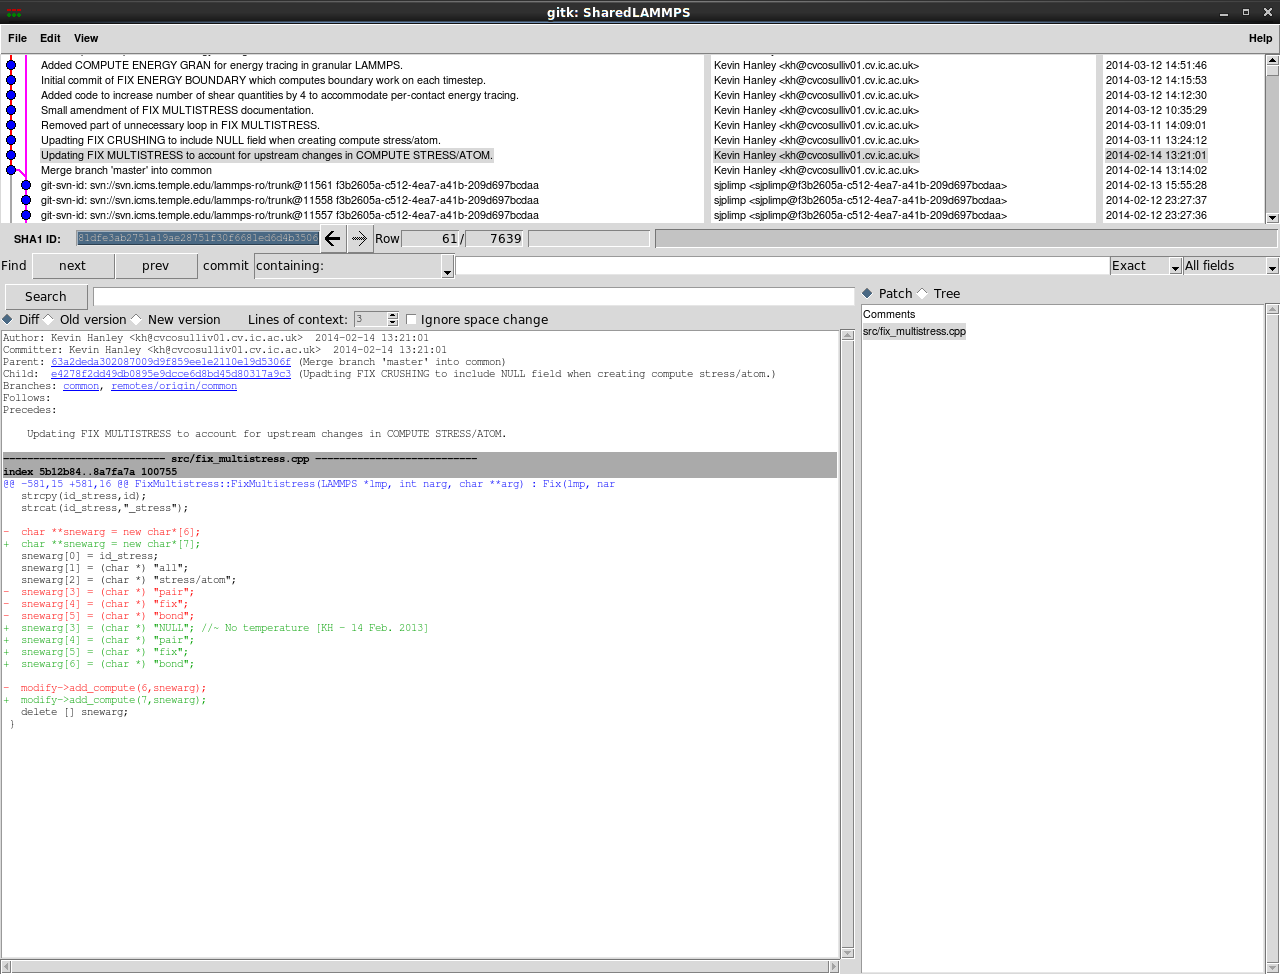
\includegraphics[width=0.95\textwidth]{Screenshot-gitk.png}
  \caption{Screenshot of \emph{gitk} showing the common branch of the local repository}\label{fig:gitk}
\end{figure}

\subsection{Adding a new file to the common repository}\label{ssec:anfcr}
We can add a new empty file, ``test.txt'', to the GRANULAR directory of the common branch of our local repository as follows:
\begin{alltt}
[user gitLAMMPS]\$ cd src/GRANULAR/
[user GRANULAR]\$ touch test.txt
\end{alltt}
If you query the status of the branch using \texttt{git status}, git will tell you that untracked files are present but it won't do anything about it:
\begin{alltt}
[user gitLAMMPS]\$ git status
# On branch common
# Untracked files:
#   (use "git add <file>..." to include in what will be committed)
#
#	test.txt
nothing added to commit but untracked files present (use "git add" to track)
\end{alltt}
You need to add the file yourself using the \texttt{git add} command. Afterwards\ldots
\begin{alltt}
[user gitLAMMPS]\$ git add test.txt
[user gitLAMMPS]\$ git status
# On branch common
# Changes to be committed:
#   (use "git reset HEAD <file>..." to unstage)
#
#	new file:   test.txt
\end{alltt}
The final step is committing the changes by running \texttt{git commit -a}, which ensures the file will henceforth be tracked by git. In the process of committing the file, you are required to add a commit message: a brief description of the changes being committed to the repository. Try to make your commit messages vaguely descriptive. The commit messages are added using the vi editor (see basics of vi below).
\begin{alltt}
[user GRANULAR]\$ git commit -a
[common a97c50b] Adding a new file with this commit message.
 0 files changed, 0 insertions(+), 0 deletions(-)
 create mode 100644 src/GRANULAR/test.txt
\end{alltt}
\noindent\hrulefill\\
\textit{\textbf{Basics of adding a commit message with vi}
\begin{enumerate}
  \item Change to the insert mode of vi by pressing <I>.
  \item Type your message as normal.
  \item Press the <ESC> key to exit text insertion mode.
  \item Type ``:wq'' to write out and quit vi.
\end{enumerate}
}\noindent\hrulefill\\
In summary, adding a new file to git is a two-step process (after moving the file to the appropriate directory in gitLAMMPS):
\begin{alltt}
[user gitLAMMPS]\$ git add test.txt
[user gitLAMMPS]\$ git commit -a
\end{alltt}

\subsection{Modifying an existing file}
Modifying an existing file is easier than adding a new file. Add some text to test.txt, save and close the file. We commit the change as before, writing a suitable commit message:
\begin{alltt}
[user GRANULAR]\$ git commit -a
[common 0ab5959] Added a line to this test file.
 1 files changed, 1 insertions(+), 0 deletions(-)
\end{alltt}

\subsection{Deleting a file from the common repository}\label{ssec:dfcr}
This is basically the reverse of adding a file; simply replace \texttt{git add} with \texttt{git rm}:
\begin{alltt}
[user GRANULAR]\$ git rm test.txt
rm 'src/GRANULAR/test.txt'
[user GRANULAR]\$ git commit -a
[common c7c3787] Deleted test file.
 1 files changed, 0 insertions(+), 1 deletions(-)
 delete mode 100644 src/GRANULAR/test.txt
\end{alltt}

The log for the complete add\slash modify\slash delete sequence of operations looks as follows:
\begin{alltt}
[user GRANULAR]\$ git log
commit c7c3787bbbf2fb71670e0f509ce004c2ad9cc970
Author: \sout{Kevin Hanley} <\sout{kh@cvcosulliv01.cv.ic.ac.uk}>
Date:   Thu Mar 13 15:08:25 2014 +0000

    Deleted test file.

commit 0ab59598a3b19f8f4ca3f0ae9566dba744783189
Author: \sout{Kevin Hanley} <\sout{kh@cvcosulliv01.cv.ic.ac.uk}>
Date:   Thu Mar 13 15:06:00 2014 +0000

    Added a line to this test file.

commit a97c50b8abd35b266308a314f9ff434f0b3511a4
Author: \sout{Kevin Hanley} <\sout{kh@cvcosulliv01.cv.ic.ac.uk}>
Date:   Thu Mar 13 14:55:02 2014 +0000

    Adding a new file with this commit message.
\ldots\hspace*{10em}\ldots\hspace*{10em}\ldots
\end{alltt}

\section{Interaction of local and remote repositories}\label{sec:ilrr}
The local repository has been created on a workstation in \prettyref{sec:clr} and we have seen how to make changes to the common branch in \prettyref{sec:vcc}. We now need to learn how to transfer our changes to the remote repository on Bitbucket (\prettyref{ssec:pclcrc}) and how to update the master branch, both in the local (\prettyref{ssec:ulmb}) and remote (\prettyref{ssec:urmb}) repositories.

\subsection{Pushing changes from local common branch to remote common branch}\label{ssec:pclcrc}
The easiest way to transfer our changes from local to remote is to use the \texttt{git push} command:
\begin{alltt}
[user \(\sim\)]\$ cd \(\sim\)/Documents/gitLAMMPS/
[user gitLAMMPS]\$ git push origin common
\end{alltt}
\ldots and enter your password when requested. The arguments of git push give the destination (origin) and the branch to be pushed. If there are no changes to commit, you will see the message ``\texttt{Everything up-to-date}''; otherwise you will see a summary of the changes made to the remote common branch.

\subsection{Updating the local master branch}\label{ssec:ulmb}
In order to update the master branch by dragging in the developments made by the upstream developers at Sandia, we create a new alias to a remote destination: the LAMMPS repository at Temple University set up by Axel Kohlmeyer (described at \url{http://lammps.sandia.gov/download.html}). Use the \texttt{git remote} command previously seen in \prettyref{ssec:cdrr} to add a new remote called 'upstream'. 
\begin{alltt}
[user \(\sim\)]\$ cd \(\sim\)/Documents/gitLAMMPS/
[user gitLAMMPS]\$ git remote add upstream http://git.icms.temple.edu/lammps-ro.git
[user gitLAMMPS]\$ git remote -v
origin	https://\sout{USERNAME}@bitbucket.org/granlammps/gitlammps.git (fetch)
origin	https://\sout{USERNAME}@bitbucket.org/granlammps/gitlammps.git (push)
upstream	http://git.icms.temple.edu/lammps-ro.git (fetch)
upstream	http://git.icms.temple.edu/lammps-ro.git (push)
\end{alltt}
Now the \texttt{git pull} command can be used to update the master branch of the local repository.
\begin{description}
 \item[\textcolor{red}{WARNING:}] \bfseries\MakeUppercase{It is essential that you switch to the master branch \emph{before} running \texttt{git pull}. The \texttt{git pull} command is potentially dangerous as it always merges into the branch which is currently checked out, whatever that happens to be.}
\end{description}
\begin{alltt}
[user \(\sim\)]\$ cd \(\sim\)/Documents/gitLAMMPS/
[user gitLAMMPS]\$ git checkout master
[user gitLAMMPS]\$ git pull upstream master
\end{alltt}
This may take a few minutes to run so be patient. The output in the terminal window will list the files that have been modified since the branch was last updated, indicate the degree of change to each of these files, tell you the numbers of files changed\slash insertions\slash deletions, and list any files which have been added\slash deleted:
\begin{alltt}
From http://git.icms.temple.edu/lammps-ro
 * branch            master     -> FETCH_HEAD
Updating 039af55..be64063
Fast-forward
 doc/Manual.html                 |    4 +-
 doc/Manual.txt                  |    4 +-
 src/neighbor.cpp                |  140 ++++++++++++++++++++++++---------------
\ldots\hspace*{10em}\ldots\hspace*{10em}\ldots
 src/version.h                   |    2 +-
 22 files changed, 229 insertions(+), 118 deletions(-)
 create mode 100644 src/rcb.cpp
 create mode 100644 src/rcb.h
\end{alltt}

\subsection{Updating the remote master branch}\label{ssec:urmb}
Updating the remote master branch on Bitbucket is a two-step process:
\begin{enumerate}
  \item Update the local master branch as described in \prettyref{ssec:ulmb}.
  \item Use \texttt{git push} to transfer changes made in the local master branch to the remote master branch, the commands for which are given below:
\end{enumerate}
\begin{alltt}
[user \(\sim\)]\$ cd \(\sim\)/Documents/gitLAMMPS/
[user gitLAMMPS]\$ git push origin master
Counting objects: 61, done.
Delta compression using up to 4 threads.
Compressing objects: 100\% (24/24), done.
Writing objects: 100\% (35/35), 719.86 KiB, done.
Total 35 (delta 27), reused 29 (delta 21)
To https://\sout{USERNAME}@bitbucket.org/granlammps/gitlammps
   f89510a..ebc7b99  master -> master
\end{alltt}

\section{Merging master branch into common branch}
Periodically merging the master branch into the common branch is the mechanism by which our version of LAMMPS, including all of our in-house additions and modifications, is kept up-to-date with the upstream LAMMPS distribution. This approach has worked well in the past and is infinitely preferable to trying to update the code manually. 

There is, however, a potential problem. A change made to the upstream code may affect some of the added\slash modified files in our version of LAMMPS. To give a simple example, the syntax of compute\_stress\_atom.cpp was changed by the main developers in February 2014 to add a temperature argument. Two files in our version of LAMMPS, fix\_multistress.cpp and fix\_crushing.cpp, implicitly set up a stress compute by calling ComputeStressAtom; this meant that both of these files needed updating. Another example is that changes made to dump\_custom.\{cpp\slash h\} usually necessitate similar changes in dump\_vtk.\{cpp\slash h\}. The only way to know the knock-on effects of upstream changes is to have an intimate knowledge of our version of LAMMPS. Updating the code by doing a merge without this understanding will almost certainly lead to problems.

Merging operations can be done only with the local repository. Even if this were not the case, it is the most sensible approach as if anything goes wrong (though it shouldn't if you follow this procedure), you can easily delete and recreate the local repository by cloning the remote repository (\prettyref{sec:clr}).

\subsection{Before merging}\label{ssec:bm}
In preparation for merging the master branch into the common branch, this sequence is recommended:
\begin{enumerate}
  \item Get the local master branch up-to-date (\prettyref{ssec:ulmb}).
  \item Switch to the common branch of the local repository. Use \texttt{gitk} (\prettyref{ssec:vpcr}) to identify the date and time of the last merged upstream commit and make a note of this. For example, the last upstream commit shown on \prettyref{fig:gitk} is ``\textit{2014-02-13 15:55:28}''.
  \item Switch to the master branch. Look carefully at each of the upstream changes that have been made since this date. Make note of any upstream changes that will require some code modification on your part. If the number of files requiring modification is large (say, more than five) and\slash or there are a huge number of upstream commits (likely if you haven't merged in the last month), it may be worthwhile doing several smaller merges rather then one enormous one.
\end{enumerate}
After assiduously following these steps, you will have a list of files that will need modification post-merge. You will also know whether it would be better to do one merge or to divide the merge into several smaller ones.

\subsection{Doing a merge}
The command to use, unsurprisingly, is \texttt{git merge}.
\begin{description}
 \item[\textcolor{red}{WARNING:}] \bfseries\MakeUppercase{Make certain that you check out the common branch before merging.}
\end{description}
As the warning states, it is of paramount importance that you are in the common branch as \texttt{git merge} merges another branch into the current one that is checked out, whatever that may be. To do a full merge of all changes:
\begin{alltt}
[user \(\sim\)]\$ cd \(\sim\)/Documents/gitLAMMPS/
[user gitLAMMPS]\$ git checkout common
[user gitLAMMPS]\$ git merge master
\end{alltt}
One of two things will occur. Either the merge will work perfectly or else a message about a \emph{merge conflict} will be returned. If the merge works perfectly, git automatically commits the file changes so you don't need to do this yourself. Dealing with merge conflicts is the subject of \prettyref{ssec:rmc}. You need to make the necessary modifications to the files identified in \prettyref{ssec:bm} regardless of whether a merge conflict occurs or not.

It is also possible to do a partial merge; this means that you merge only up to a specified commit on the master branch. On the master branch, take note of the relevant \emph{commit ID}. A commit ID is a long alphanumeric string, unique to each commit, which looks like this: \texttt{c7c3787bbbf2fb71670e0f509ce004c2ad9cc970}. The commit ID can be found easily using \texttt{git log} or \texttt{gitk} (as ``SHA1 ID'' on the left-hand side). A partial merge can be done by appending this commit ID to the usual \texttt{git merge} command instead of specifying a branch:
\begin{alltt}
[user \(\sim\)]\$ cd \(\sim\)/Documents/gitLAMMPS/
[user gitLAMMPS]\$ git checkout common
[user gitLAMMPS]\$ git merge \sout{c7c3787bbbf2fb71670e0f509ce004c2ad9cc970}
\end{alltt}

\subsection{Resolving merge conflicts}\label{ssec:rmc}
Suppose that a merge conflict occurs (caused by ``pair.cpp''):
\begin{alltt}
[user gitLAMMPS]\$ git merge master
Auto-merging src/fix.h
Auto-merging src/pair.cpp
CONFLICT (content): Merge conflict in src/pair.cpp
Auto-merging src/pair.h
Automatic merge failed; fix conflicts and then commit the result.
\end{alltt}
This message indicates that some problem has arisen when auto-merging src/pair.cpp. We can also summarise all of the files affected by the merge and their status using the \texttt{git status} command with the optional ``-s'' (for ``short'') switch:
\begin{alltt}
[user gitLAMMPS]\$ git status -s
M  doc/Manual.html
\ldots\hspace*{10em}\ldots\hspace*{10em}\ldots
UU src/pair.cpp
\ldots\hspace*{10em}\ldots\hspace*{10em}\ldots
M  src/version.h
\end{alltt}
Any files preceded by ``M'' have been merged without conflict; files preceded by ``UU'' contain a conflict. Why has a conflict occurred in pair.cpp? This is what the relevant part of the file used to look like in the common branch (and what pair.cpp still looks like in the common branch of the remote repository, if everything is up-to-date):

\noindent\textcolor{customblue}{\rule{8cm}{0.8pt}}
\begin{alltt}
  vatom = NULL;

  datamask = ALL_MASK;
  datamask_ext = ALL_MASK;

  /*~ Added to initialise the status of the rolling resistance
    model as disabled [KH - 23 October 2013]*/
  rolling = 0;

  //~ Initialise at 1 [KH - 25 October 2013]
  model_type = 1;

  /*~ Initialise the status of per-contact energy tracing as
    inactive [KH - 6 March 2014]*/
  trace_energy = 0;
\end{alltt}
\noindent\textcolor{customblue}{\rule{8cm}{0.8pt}}

The upstream version of pair.cpp in the master branch (which, remember, we are trying to merge with the code shown immediately above) looks like this:

\noindent\textcolor{customblue}{\rule{8cm}{0.8pt}}
\begin{alltt}
  vatom = NULL;

  // CUDA and KOKKOS per-fix data masks

  datamask = ALL_MASK;
  datamask_ext = ALL_MASK;

  execution_space = Host;
  datamask_read = ALL_MASK;
  datamask_modify = ALL_MASK;
\end{alltt}
\noindent\textcolor{customblue}{\rule{8cm}{0.8pt}}

Clearly, four new lines (one comment and three lines of code) have been added by the upstream developers. The conflict has occurred because although git is smart enough to insert the comment at the correct place, it is confused by the disparity at the end of the code section. After the merge conflict, pair.cpp in the local common branch looks like this:

\noindent\textcolor{customblue}{\rule{8cm}{0.8pt}}
\begin{alltt}
  vatom = NULL;

  // CUDA and KOKKOS per-fix data masks

  datamask = ALL_MASK;
  datamask_ext = ALL_MASK;

<<<<<<< HEAD
  /*~ Added to initialise the status of the rolling resistance
    model as disabled [KH - 23 October 2013]*/
  rolling = 0;

  //~ Initialise at 1 [KH - 25 October 2013]
  model_type = 1;

  /*~ Initialise the status of per-contact energy tracing as
    inactive [KH - 6 March 2014]*/
  trace_energy = 0;
=======
  execution_space = Host;
  datamask_read = ALL_MASK;
  datamask_modify = ALL_MASK;
>>>>>>> master
\end{alltt}
\noindent\textcolor{customblue}{\rule{8cm}{0.8pt}}

Wherever there is a merge conflict, git inserts \emph{markers} around the relevant code in the following way:
\begin{alltt}
<<<<<<< HEAD
  Code from file in common version.
=======
  Code from upstream file in master version.
>>>>>>> master
\end{alltt}
The code won't compile while these markers are present. This must be resolved manually by opening the file in a suitable editor (such as Emacs; if you use a Windows OS, refrain from using Notepad\slash Wordpad), correcting the code including deleting the markers, then saving and closing the file. After the author did this, pair.cpp looked like the following:

\noindent\textcolor{customblue}{\rule{8cm}{0.8pt}}
\begin{alltt}
  vatom = NULL;

  // CUDA and KOKKOS per-fix data masks

  datamask = ALL_MASK;
  datamask_ext = ALL_MASK;

  execution_space = Host;
  datamask_read = ALL_MASK;
  datamask_modify = ALL_MASK;

  /*~ Added to initialise the status of the rolling resistance
    model as disabled [KH - 23 October 2013]*/
  rolling = 0;

  //~ Initialise at 1 [KH - 25 October 2013]
  model_type = 1;

  /*~ Initialise the status of per-contact energy tracing as
    inactive [KH - 6 March 2014]*/
  trace_energy = 0;
\end{alltt}
\noindent\textcolor{customblue}{\rule{8cm}{0.8pt}}

After resolving the merge conflict, we need to \emph{add} the file to git again (which is slightly counter-intuitive) to change the status of the file from ``UU'' to ``M''. Finally we need to commit the merge, a step which is necessary only when a merge conflict has occurred:
\begin{alltt}
[user gitLAMMPS]\$ git add src/pair.cpp
[user gitLAMMPS]\$ git status -s
\ldots\hspace*{10em}\ldots\hspace*{10em}\ldots
M  src/pair.cpp
\ldots\hspace*{10em}\ldots\hspace*{10em}\ldots
[user gitLAMMPS]\$ git commit -a
\end{alltt}

\subsection{After merging}
\begin{enumerate}
  \item After merging, the priority is to make the necessary modifications to the files identified in \prettyref{ssec:bm} and commit these changes.
  \item Then try compiling a serial build of LAMMPS. If problems arise during compilation, these must be fixed before continuing any further. The common branch of LAMMPS in the remote repository must \emph{always} compile; what you do in the local repository on your own workstation is your own business.
  \item Once the code compiles and all seems to be well, push the updated common branch to the remote repository as described in \prettyref{ssec:pclcrc}.
\end{enumerate}

\end{document}